\documentclass[aspectratio=169]{beamer}
\mode<presentation>

% packages
\usepackage[utf8]{inputenc}
\usepackage{lmodern}
\usepackage{textpos}
\usepackage{pdfpages}
\usepackage{multicol}
\usepackage{amsmath}
\usepackage{amssymb}
\usepackage[most]{tcolorbox}
\usepackage{enumitem}
\setlist[itemize,1]{label={\fontfamily{cmr}\fontencoding{T1}\selectfont\textbullet}}
\setlist[itemize,2]{label={\fontfamily{cmr}\fontencoding{T1}\selectfont\textopenbullet}}

% inser here your presentation basic info
\newcommand{\mysession}{SS16b}
\newcommand{\mysessionname}{Registering the Universe at the highest spatial accuracy}
\newcommand{\mytitle}{(Re)solving the riddle about the size of GRB170817A through global VLBI observations}
\newcommand{\myshorttitle}{(Re)solving the riddle about the size of GRB170817A}
\newcommand{\myname}{Om Sharan Salafia}
\newcommand{\myshortname}{Om S. Salafia}
\newcommand{\myinstitutes}{INAF -- Osservatorio Astronomico di Brera, Milan, Italy\\ INFN -- Sezione di Milano-Bicocca, Milan, Italy}

% template tweaks
\definecolor{EAS_blue}{RGB}{32, 104, 142}
\definecolor{EAS_orange}{RGB}{249, 207, 116}

\usetheme{Rochester}
\setbeamertemplate{blocks}[rounded][shadow=false]
\usecolortheme{beetle}

% logo
\addtobeamertemplate{headline}{}{%
\begin{textblock*}{100mm}(.85\textwidth,-1.5cm)

\includegraphics[width=2cm]{figures/EAS_2020_logo.png}
\end{textblock*}}

% ``keys''
\addtobeamertemplate{headline}{}{%
\begin{textblock*}{100mm}(0.0\textwidth,-1.5cm)

\includegraphics[width=0.8cm]{figures/EAS_2020_keys.png}
\end{textblock*}}

% remove navigation symbols
\setbeamertemplate{navigation symbols}{}

% set the correct footline colors
\setbeamercolor{myfootlinecolor}{fg=EAS_blue,bg=EAS_orange}

% your footline
\makeatother
\setbeamertemplate{footline}{%
  \leavevmode%
  \hbox{\begin{beamercolorbox}[wd=\paperwidth,ht=3ex,dp=1.125ex,leftskip=.3cm,rightskip=.3cm]{myfootlinecolor}%
  \insertpagenumber \hfill \myshortname\  -- \myshorttitle  \hfill EUROPEAN ASTRONOMICAL SOCIETY ANNUAL MEETING 
  \end{beamercolorbox}}%
}
\makeatletter

% set up colors
\setbeamercolor{normal text}{fg=black}
\setbeamercolor{background canvas}{bg=white}

\setbeamercolor{frametitle}{fg=EAS_orange}
\setbeamercolor{frametitle}{bg=EAS_blue}
\setbeamercolor{footline}{bg=EAS_orange,fg=EAS_blue}
\setbeamercolor{block body alerted}{bg=white_orange}

\usefonttheme{professionalfonts}

\AtBeginSubsection

\setlength{\unitlength}{\textwidth}


%%%%%%%%%%%%%%%%%%%%%%%%%%%%%%%%%%%%%%%%%%%%%%%%%%%%%%%%%%%%%%%%%%%%%%%%%%%%%%%%%%

\begin{document}

%%%%%%%%%%%%%%%%%%%% TITLE SLIDE %%%%%%%%%%%%%%%%%%%%%%%%%%%%%%%%%%%%%%%%%%%%%%%%%

% everything should work out automatically here, but you can tweak whatever you want

{
\usebackgroundtemplate{
\includegraphics[width=\paperwidth]{figures/EAS_2020_title_bkg.png}}%

\begin{frame}[plain,noframenumbering,t]

\begin{columns}[t]
 \column{0.35\textwidth}
   \vspace{10pt}
   
   \centering
   
\includegraphics[width=0.9\columnwidth]{figures/EAS_2020_logo.png}
   
   \Large \textcolor{white}{European Astronomical Society Annual Meeting}\\
   
   \flushleft \normalsize\vspace{-8pt}\textcolor{white}{{\fontfamily{pag}\selectfont EWASS}}
   
   \centering
   
   \Large\vspace{10pt}\textcolor{EAS_orange}{\mysession}\\
   \normalsize\textcolor{EAS_orange}{\mysessionname}
   
 \column{0.65\textwidth}
 %\vspace{10pt}
 
 \centering
 
 \Large \textcolor{white}{\mytitle}
 
 \footnotesize \textcolor{white}{by}
 
 \normalsize \textcolor{EAS_orange}{\myname}\\[4pt]
 
 \footnotesize \textcolor{EAS_orange}{\myinstitutes}\\[8pt]

%I've put my logos here, but these are not mandatory
%\includegraphics[width=0.15\textwidth]{figures/logoOABHiRes-white.png}\hspace{10pt}
%\includegraphics[width=0.12\textwidth]{figures/INAF_logo_negative.png}\hspace{10pt}
%\includegraphics[width=0.12\textwidth]{figures/infn_logo1_negative.png}

\end{columns}

\end{frame}
\addtocounter{framenumber}{-1}
}


%%%%%%%%%%%%%%%%%%%%%%%%%%%%%%%%%%%%%%%%%%%% PRESENTATION STARTS HERE %%%%%%%%%%%%%%%%%%%%%%%%%%

\begin{frame}
 \frametitle{Intro: gravitational waves (GW)}

 \begin{columns}
 
 \column{0.55\textwidth}
    \centering
    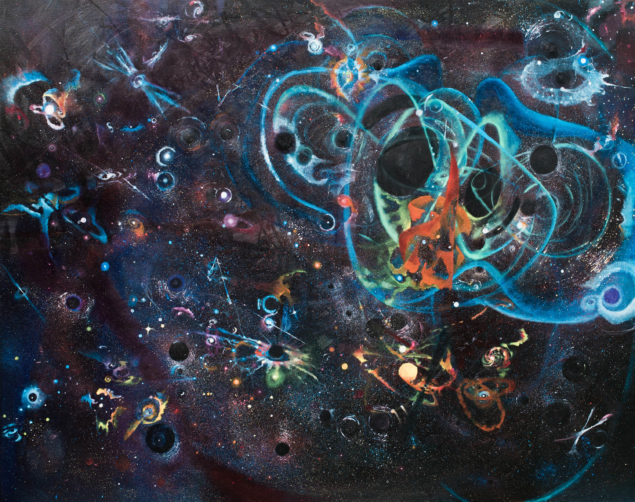
\includegraphics[height=0.9\textheight]{figures/GW-Penelope-Cowley.jpg}

    \tiny [``Gravitational Waves'', artwork by Penelope Cowley]

\column{0.45\textwidth}
 
 \centering
 
 \alert{Perturbations} of space-time metric (a.k.a.~gravity)\\[10pt]
 
 Produced by mass-energy distributions whose \alert{quadrupole} moment accelerates\\[10pt]
 
 Propagate at \alert{$c$} (experimentally!)\\[10pt]
 
 Cause dilation/contraction \alert{perpendicular} to propagation\\[10pt]
 
 \end{columns}

\end{frame}

\end{document}
